\documentclass[a4paper, 11pt]{article}
\usepackage[utf8]{inputenc}
\usepackage[parfill]{parskip}
\usepackage{graphicx}	
\usepackage{wrapfig}
\usepackage{amssymb}
\usepackage{censor}
\usepackage{ulem}
\usepackage{boxedminipage}
\usepackage{tocloft}
\usepackage{setspace}
\usepackage{hyperref}

\hypersetup{
pdftitle = {SCP - Secure, Contain, Protect},
pdfkeywords = {scp,creepypasta,weird,supernatural},
}

%custom font
\usepackage{fontspec}
\setmainfont[
    ItalicFont={Underwood Champion},
    ItalicFeatures={FakeSlant=0.2}
  ]{Underwood Champion}

%Supposed to be used for line spacing between the items, not the entire block
\setlength\cftbeforetoctitleskip{10pt}
\setlength\cftaftertoctitleskip{0pt}

%custom commands
\newcommand{\lb}{\ensuremath{[}}
\newcommand{\rb}{\ensuremath{]}}
\newcommand{\degree}{$^{\circ}$}
\newcommand{\redacted}{\lb REDACTED\rb}
\newcommand{\expunged}{\lb DATA EXPUNGED\rb}
\newcommand{\classified}{\lb CLASSIFIED\rb}
\newcommand{\toclesssection}[1]{\section*{#1}\addtocounter{section}{1}}
\newcommand{\fakebold}[1]{{\addfontfeatures{FakeBold}#1}}
\renewcommand{\textbf}[1]{{\addfontfeatures{FakeBold}#1}}

%Generate random numbers for the background image selection
\usepackage{lcg}
\reinitrand[counter=sec,first=1,last=3]

%Backgroundimage
\usepackage{eso-pic}
\newcommand\BackgroundPic{
\put(0,0){
\parbox[b][\paperheight]{\paperwidth}{%
\vfill
\centering
\rand\includegraphics[width=\paperwidth,height=\paperheight,
keepaspectratio]{img/bg_\thesec.pdf}%
\vfill
}}}



\begin{document}

\AddToShipoutPicture{\BackgroundPic}

\begin{center}

\includegraphics[scale=0.3]{img/logo_bwu.png}
\end{center}

\renewcommand\contentsname{}
\begin{spacing}{0.1}
\tableofcontents
\end{spacing}
\newpage

\toclesssection{SCP 001 - Awaiting De-classification \lb BLOCKED\rb}
\addcontentsline{toc}{section}{SCP 001 - Awaiting De-classification \lb BLOCKED\rb}
\lb BLOCKED\rb
\toclesssection{SCP 002 - The "Living" Room}
\addcontentsline{toc}{section}{SCP 002 - The "Living" Room}
\textbf{Item \#:} SCP-002

Object Class: Euclid

\begin{wrapfigure}{l}{7,5cm}
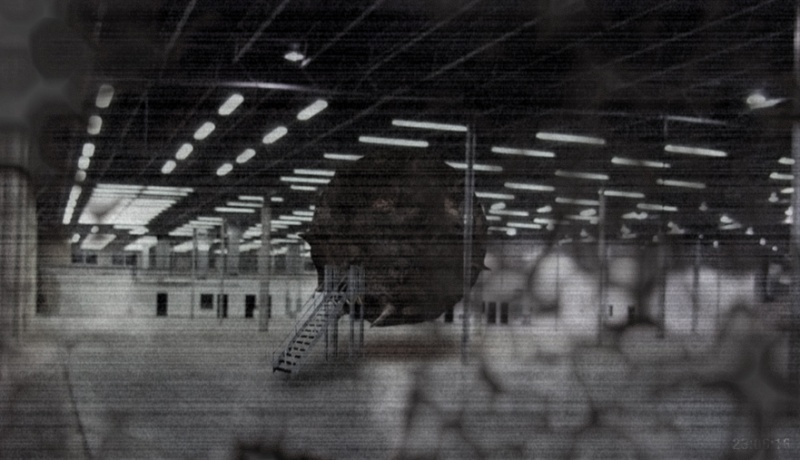
\includegraphics[scale=0.255]{scp/002.jpg}
\end{wrapfigure}

Special Containment\linebreak Procedures: SCP-002 is to remain connected to a suitable power supply at all times, to keep it in what appears to be a recharging mode. In case of electrical outage, the emergency barrier between the object and the facility is to be closed and the immediate area evacuated. Once facility power is re-established, alternating bursts of X-ray and ultraviolet light must strobe the area until SCP-002 is re-affixed to the power supply and returned to recharging mode. Containment area is to be kept at negative air pressure at all times.

Teams including a minimum of two (2) members are required within 20 meters of SCP-002 or its containment area. Personnel should maintain physical contact with one another at all times to confirm there is another person present as perception may be dulled, skewed, or influenced by proximity to the object.

No personnel below Level 2 are permitted within SCP-002. This requirement may be waived via written authorization from two (2) off-site O5-level administrators. Command staff issued such a waiver must be escorted by at least five (5) Level 3 Security personnel for the duration of their contact and must temporarily surrender their rank and security clearance. Following contact, command staff will be escorted at least 5 km from SCP-002 to undergo a seventy-two (72)-hour quarantine and psychological evaluation. If deemed fit for return to duty by psych staff, rank and security clearance may be restored when quarantine expires.

Description: Refer to the Mulhausen Report \lb cross-ref:\linebreak document00.023.603\rb for details related to object's discovery. SCP-002 resembles a tumorous, fleshy growth with a volume of roughly 60 m$^3$ (or 2000 ft$^3$). An iron valve hatch on one side leads to its interior, which appears to be a standard low-rent apartment of modest size. One wall of the room possesses a single window, though no such opening is visible from the exterior. The room contains furniture which, upon close examination, appears to be sculpted bone, woven hair, and various other biological substances produced by the human body. All matter tested thus far show independent or fragmented DNA sequences for each object in the room.

Reference: To date, subject has been responsible for the disappearances of seven personnel. It has also in its time at the facility further furnished itself with two lamps, a throw rug, a television, a radio, a beanbag chair, three books in an unknown language, four children's toys, and a small potted plant. Tests with a variety of lab animals including higher primates have failed to provoke a response in SCP-002. Cadavers as well fail to produce any effect. Whatever process the subject uses to convert organic matter into furnishings is apparently only facilitated by the introduction of living humans.

\begin{bordered}{Mulhausen Report \lb 00.023.603\rb}

The following is a brief report detailing the discovery of SCP-002

Subject was discovered in a small crater in northern Portugal where it struck the Earth from orbit. Encased in a shell of thick rock, the fleshy exterior of the object was exposed by the impact. A native farmer happened upon the site and reported his findings to the village elder. Subject gained SCP attention when a Level 4 agent posted in the area detected a small radioactive anomaly generated by the object.

A collection squad of SCP security personnel led by General Mulhausen was immediately dispatched to the area where they quickly secured the subject in a large container and performed initial testing with subjects recruited from the nearby village. Three men individually sent into the structure subsequently disappeared. Upon discovering this deadly property of the subject, General Mulhausen issued a Level 4a Termination Order of any witnesses (roughly 1/3 of the village) to ensure no outside knowledge of the object and initiated its transport to SCP facility \expunged.

During preparation for transport, four SCP security personnel were inexplicably drawn inside the object where they too immediately disappeared. Following inspection, it appeared as if the object had "grown" several new furnishings and was beginning to look like the interior of an apartment room. General Mulhausen immediately ordered the requisition of several Class III HAZMAT suits for the remaining security team members, who proceeded to lift the container onto a waiting freight ship for transport to the SCP containment facility.

\expunged

\expunged

Following the termination of General Mulhausen, SCP-002 was re-secured by SCP staff and brought into special containment in \classified, where it currently resides. Command staff with any authority below Level 2 have been denied access to the SCP-002 container without prior approval of at least two Level O5 command staff after the Mulhausen incident.

\end{bordered}

\toclesssection{SCP 003 - Biological Motherboard}
\addcontentsline{toc}{section}{SCP 003 - Biological Motherboard}
Item \#: SCP-003

Object Class: Euclid

\begin{wrapfigure}{l}{7,5cm}

\includegraphics[scale=0.34]{scp/003.jpg}
\end{wrapfigure}

Special Containment\linebreak Procedures: SCP-003 is to be maintained at a constant temperature of no less than 35\degree C and ideally kept above 100\degree C. In event of total power failure, assigned personnel must use their body heat to keep SCP-003-1 above the critical temperature. All personnel who have come in physical contact with SCP-003-1 are to immediately report for sterilization afterwards.

SCP-003-1 must not be removed from SCP-003-2 except in case of emergency procedures detailed above. Any significant change in SCP-003-2's rune activity (including pattern, frequency, or color) should be reported within three (3) hours of occurrence. Cessation of rune activity must be reported immediately. SCP-003-2 must be supplied with power via the source designated Generator 003-IX at all times; refer to attached documentation for details.

Description: SCP-003 was located by remote viewing team SRV-04 Beta (see attached documents). SCP-003 consists of two related components of separate origin, referred to as SCP-003-1 and SCP-003-2.

SCP-003-1 appears to be composed of chitin, hair, and nails of unknown biology similar to \redacted, arranged in a configuration similar to that of a computer motherboard. Testing reveals SCP-003-1 to predate earliest known circuit boards by \redacted. SCP-003-1 is considered sentient but not actively dangerous except under certain conditions (see addenda and attached documents).

SCP-003-1 was found on a stone tablet, SCP-003-2, on which it currently resides. The runes on SCP-003-2 are not part of any known language, and flicker with pale tones. These are effects of communication, interpretable by \expunged.

Analysis has shown that SCP-003-1 and SCP-003-2 have different origins. SCP-003-2 is controlled by a (non-biological) internal computer, the contents of which are mostly inaccessible without risk of damaging SCP-003-2. SCP-003-2 is capable of controlled emissions of radiation, including heat and \redacted. It is considered probable that SCP-003-2 was created for the purpose of containing SCP-003-1. Methods detailed in Addendum 003-01 have allowed access to some data contained in SCP-003-2; while interpretation is not conclusive, contents may refer to a past and/or potential future \censor{XX}-class restructuring event caused by SCP-003-1.

SCP-003-2 contains an internal power source of \linebreak \expunged, which appears to have been losing power since \censor{XXXXXXXXXX} before discovery by SRV-04 Beta. It appears possible that SRV-04 Beta was deliberately contacted by SCP-003-2 via \expunged Other organizations have also been alerted to SCP-003's existence, possibly by similar means. Despite this activity, SCP-003-2 does not appear to be sentient, based on \redacted and its lack of reaction to \redacted including M03-Gloria procedures.

When SCP-003 drops below the temperature of 35\degree C, both components react.

First, SCP-003-1 enters a growth state characterized by an exponential increase in mass. This growth state consists of two stages. In both stages, SCP-003-1 partially fuels its growth by converting matter around it, starting with any surrounding inorganic material, including atmospheric elements, then nonliving organic material, including cells of dead skin, hair, chitin, enamel, keratin, and other biological materials.

The first stage is the 'default' stage; the second stage begins when SCP-003-1 comes in contact with living organic material. In its second stage, SCP-003-1 may pause, slow or change its growth, and will also reprocess inorganic and nonliving organic elements into functionally similar structures while \expunged

While growth is consistent in the first stage, in the second stage SCP-003-1's growth rate is diminished by 20-90\% so long as SCP-003-1 remains in contact with living organic material. The percentage is determined by the complexity of the organism(s) in contact with SCP-003-1; as confirmed by \redacted readings, SCP-003-1 appears to devote a large amount of processing power to analysis of living organic material.

During each of SCP-003-1's growth stages, SCP-003-2 releases bursts of radiation that temporarily inhibit SCP-003-1's growth, or reverse this growth when the temperature of SCP-003-1 rises above 100\degree C. Similar radiation emissions may be produced via \expunged.

Addendum 003-01: Acting on information gathered from linguistic analysis of SCP-003-2's runes and \expunged, Research Team M03-Gloria has managed to establish a link between SCP-003 and \expunged for analysis of functions. SCP-003-1 must now be considered sentient, and is to be kept a minimum of 1 km from \expunged and the resulting "by-product" at all times.

Addendum 003-02: SCP-003-2's power loss has been exacerbated by the procedures performed by M03-Gloria. On orders of O5-\censor{XX}, M03-Gloria will continue procedures.

Addendum 003-03 \expunged During this process, SCP-003-1 doubled its mass and began rapid structural growth. Temperature was immediately returned to 100\degree C. Growth and mass increase of SCP-003-1 continued for 9 minutes and 6 seconds, at which time a sustained radiation spike was produced by SCP-003-2. In response, SCP-003-1 returned to its normal state in 3 minutes and 39 seconds. New growth dissolved into a dusty residue which was collected for analysis. Both SCP-003-1 and SCP-003-2 ceased all detectable activity. SCP-003-2 did not resume activity until connected \redacted external power source. SCP-003-2's runes glowed uniformly gray and did not resume normal activity for three (3) hours, and afterwards \expunged SCP-003-2 no longer appears to be able to maintain containment area at a temperature above 35\degree C without external power supplied by \redacted (designated Generators 003-III through IX).

Addendum 003-04: The procedure detailed in Addendum 003-03 was repeated, and SCP-003-1 again entered a growth state. After 10 minutes and 13 seconds, SCP-003-2 once again produced a sustained radiation spike. SCP-003-1's growth stopped for 36 seconds, then resumed at its previous pace.

On quadrupling its mass, SCP-003-1 formed a coherent outer shell and body, which initially took a form similar in shape to an ophiuroid (brittle star) of fifteen meters in diameter (including what appeared to be a central processor of three meters in diameter), formed sensory organs that appeared to scan the surrounding environment, and partially converted its containment area to \redacted. SCP-003-1 then breached containment, entering the observation gallery where nine members of M03-Gloria were present. On physical contact with team members, SCP-003-1 entered stage two of its growth, and \expunged SCP-003-1 stopped growth for 15 minutes. SCP-003-1 then resumed growth, and rearranged the component parts of the center of its form to the shape of a three-meter-tall female humanoid, with peripheral "tentacles" shifting to extrude primarily from SCP-003-1's newly formed "hair" and spine. SCP-003-1 then produced rudimentary vocalizations and \expunged

An unknown Caucasian male, later identified as \redacted, approached the compromised containment area in company of a full squad of agents. \redacted claimed to be acting on orders of O5-\censor{XX} and attempted communication with SCP-003-1. \expunged Agent \censor{XXXX} of M03-Gloria successfully restored power to SCP-003-2 and activated backup generators to return the temperature to 100\degree C. SCP-003-1 returned to its normal state in 21 minutes and 7 seconds, and was successfully re-contained without incident.

All nine members of M03-Gloria affected by SCP-003-1 were afterwards found to be physically unharmed, with no residual effects besides minor psychological trauma. The converted materials of SCP-003's former containment area did not dissolve and are now under analysis.

Addendum 003-05: In light of the previous incident, O5-\censor{XX} \expunged by joint decision of O5-\censor{XX}, O5-\censor{XX}, and O5-\censor{XX}. All M03-Gloria procedures have been indefinitely suspended.

\toclesssection{SCP 004 - The 12 Rusty Keys and the Door}
\addcontentsline{toc}{section}{SCP 004 - The 12 Rusty Keys and the Door}
\fakebold{Item \#:} SCP-004

\fakebold{Object Class:} Euclid

\begin{center}
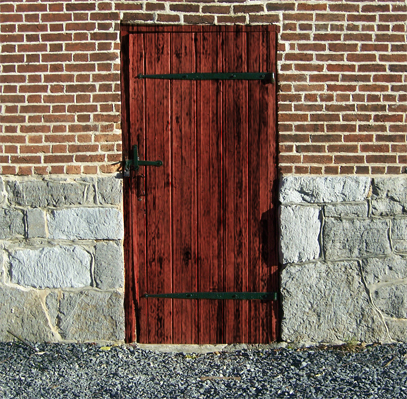
\includegraphics[scale=1.6]{scp/004.jpg}
\end{center}

\fakebold{Special Containment Procedures:} When handling items SCP-004-2 through SCP-004-13, proper procedure is vital. The items are not permitted off-site unless accompanied by two (2) Level 4 security personnel. Under no circumstances should any other component of SCP-004 be taken through SCP-004-1. The effects of doing so are as yet unknown, and the current cost of experimentation makes further research impractical. Should any of the objects contained within SCP-004-1 break containment, or the facility be breached, the keys must be brought inside and the door closed prior to activation of Site 62’s on-site warhead. Unauthorized removal of keys from the testing area is grounds for immediate termination.

Level 1 clearance is required for basic access to SCP-004-1; Level 4 clearance is required for use of SCP-004-2 to -13.

\fakebold{Description:} SCP-004 consists of an old wooden barn door (SCP-004-1) and a set of twelve (12) rusted steel keys (SCP-004-2 through SCP-004-13). The door itself is the entrance to an abandoned factory in \expunged.
\newpage

\begin{flushleft}
\fakebold{Chronological History}
\end{flushleft}
\fakebold{07/02/1949:} A group of three juveniles trespassing on federal property near \censor{XXXXXXXXXX} find the door. According to their testimony, they found a set of rusted keys in an iron lockbox and determined what door the keys unlock. The juveniles are taken into custody after they contact Sheriff \censor{XXXXXXXXXXXXXXXXX} when one of their friends (SCP-004-CAS01) goes missing.

\fakebold{07/03/1949:} Local authorities find the severed right hand of SCP-004-CAS01 eight kilometers from SCP-004-1. Other parts of SCP-004-CAS01's body are found scattered as far as 32 km from the factory. Under interrogation, the apprehended juveniles tell authorities that upon opening the door with one of the keys, SCP-004-CAS01 was torn into several pieces, each of which disappeared. At this point, the SCP Foundation takes over the investigation.

\fakebold{07/04/1949:} SCP Agent \censor{XXXXX} obtains the keys from the local authorities to begin testing. Tests show that SCP-004-2 through SCP-004-13 all fit into a single lock on the large barred door. 12 Class D personnel are assigned to test the effects of the door. Of the twelve (12) test subjects each trying a different key to enter the room, only two (2) survive. Opening the door with any key except SCP-004-7 or SCP-004-12 caused the test subjects to be torn apart in multiple directions; however, no dismembered parts were found until later. At the time of writing, only two (2) parts of each subject have been recovered (with the exception of the subject using SCP-004-\censor{X}, whose pieces were scattered in close proximity). The others have, for all intents and purposes, vanished from existence.

Of the two surviving subjects, only one (having used SCP-004-7) returned unharmed. The other came back in a near-catatonic state, able only to remove himself from the room and then collapse on the floor, and had to be restrained to prevent him from gouging out his eyes (see Appendix A: Mental Health Effects of SCP-004). The subject using SCP-004-7 said that he had entered a large room, impossibly big for the size of the attached building. After his exit, SCP-004-1 was propped open and an armed squad of Level 3 personnel entered. The size of the room is impossible to measure and the door frame and the individuals in the room are the only part of the room that can be felt or illuminated.

\fakebold{07/16/1949:} The juvenile suspects and Sheriff \censor{XXXXXXXXXXX} \censor{XXXXX} are terminated.

\fakebold{08/02/1949:} \censor{XXXXXXXXXXXXXXXXX} is declared a hazardous area "due to unexploded ordnance" and fences erected in order to prevent civilian ingress. Tests to determine safety of exposure to environment behind SCP-004-1 begin.

\fakebold{12/01/1950:} Space-time anomalies resulting from exposure to SCP-004 are confirmed. Testing is suspended until further notice.

\fakebold{07/03/19\censor{XX}:} The unaccounted-for remains of SCP-004-CAS01 appear unexpectedly outside SCP-004-1. Despite being killed decades before, the remains of SCP-004-CAS01 are not decomposed in any manner and are still warm to the touch. Blood remains uncoagulated. The remains are remanded for testing.

\fakebold{07/04/19\censor{XX}:} The unaccounted-for remains of one of the twelve (12) original test subjects appear in similar manner to those of SCP-004-CAS01. The remains have been designated SCP-004-CAS02. Records suggest that both SCP-004-CAS01 and CAS02 used SCP-004-\censor{XX}.

\fakebold{03/21/1999:} With the massive proliferation of nuclear weapons and World War III only \censor{XX} years away, construction has begun on a site inside SCP-004-1. The site is to stock supplies for \censor{XXXXXXX} person-days.

\fakebold{04/21/1999:} \censor{XXXXXXXXXXXXXXXXX} has ordered the site inside SCP-004-1 to be expanded to include emergency storage for all mobile SCP-\censor{XXX} specimens and a \censor{XX}-petabyte database for the storage of all SCP data. The facility is now referred to as Site-62.

\fakebold{09/25/2000:} Site-62 is operational. Labs and containment units are complete and can contain the most dangerous specimens. Backup of the SCP database has begun.

\fakebold{01/25/2001:} Due to time anomalies (see “Space-Time Anomalies” below), all personnel working at Site-62 are now required to reside on-site permanently. Families of personnel are to be informed that loved ones perished in an industrial accident. Cloned bodies have been prepared for funeral.

\fakebold{07/14/2003:} Massive power outage across Northeast United States and through Canada. Due to the initial failure of multiple SCP generators, Site-62 was without power for fifty-three (53) minutes. During those fifty-three (53) minutes, those on site were completely without any source of light. They reported "sensing" creatures and people, although no abnormal entities could be seen or felt. Selected facility personnel were allowed to read \censor{XXXXXXXXXXXX} (Appendix A) and said the creatures "sensed" were of humanoid size but otherwise similar to the massive green creature described.

\begin{flushleft}
\fakebold{Space-Time Anomalies}
\end{flushleft}

SCP-004 seems to propagate spatiotemporal anomalies. Personnel leaving the facility report losing time. Those who have been in the site for weeks insist that they had only been in the facility for several days, and records of work completed and supplies consumed support their claims. Other temporal anomalies involve SCP-004-2 through -13, especially the reappearance of SCP-004-CAS01 and SCP-004-CAS02 exactly \censor{XX} years after using SCP-004-\censor{XX}. \censor{XXXXXXXXXXXXXXXXXXXX} has been assigned to investigate all aspects of these time anomalies. Spatial anomalies include the impossibly large dimensions of the area opened by SCP-004-7. Similarly, the 2003 blackout incident suggests that there exists an alternate plane of existence within the same space that Site-62 occupies.

\begin{flushleft}
\fakebold{Further Notes}
\end{flushleft}

Testing on SCP-004 reveals that ten (10) of the keys open SCP-004-1 on a dimension where the laws of physics and topology are significantly different than those of our home dimension. Test subjects meeting these hostile conditions are torn apart, their body parts deposited in various locations, only three of which have been verified to be on Earth. Material deposited at two of these points appears immediately; material deposited at the third appears exactly \censor{XX} years into the future. The other seven locations are currently unknown.

Current testing focuses on two avenues of research. The first is finding ways to survive SCP-004’s hostile topologies. The second \expunged suggest that SCP-004-2 through -13 may open doors other than SCP-004-1.

\begin{flushleft}
\fakebold{Appendix A: Mental Health Effects of SCP-004-12}
\end{flushleft}

All Class D personnel using SCP-004-12 return in a catatonic state, unable to speak. Some may have enough energy left to try to claw out their eyes. Of the 16 subjects, only 4 have survived. Only one has regained speech, following long-term psychotherapy. He was able to tell the psychiatrist that he saw a massive green creature, so large that much of its body extended beyond his field of view. He reported innate fear and sudden recognition, “as if it were something buried deep in \lb his\rb primal fears,” and forced implantation of “incomprehensible” memories. Subject displays acute anterograde and retrograde amnesia.

\begin{flushleft}
\fakebold{Appendix B}
\end{flushleft}

\fakebold{Item \#:} SCP-004-14

\fakebold{Date of Discovery:} 09/02/1950

\fakebold{Origin of Object:} Object was discovered elsewhere in factory area, in the previously undiscovered manager's office.

\fakebold{Description:} Object appears as a large (182 cm X 129 cm), unvarnished wooden box. The box may be unlocked by the "safe" key, SCP-004-7, as well as five of the "unsafe" keys (see Document SCP-004-1).

Upon unlocking SCP-004-14 with SCP-004-7, the box opens automatically on hinges. The volume of the space inside is precisely five times greater than the outer dimensions imply. Items placed within while the lid remains open do not affect the weight or any other properties of the box. When the lid is closed and locked, however, all items inside vanish irretrievably. Personnel locked inside the box are also irretrievable, although losing personnel in this fashion appears to affect significantly the dreams experienced by \expunged.
\toclesssection{SCP 005 - Skeleton Key}
\addcontentsline{toc}{section}{SCP 005 - Skeleton Key}
\fakebold{Item \#:} SCP-005

\fakebold{Object Class:} Safe

\begin{center}

\includegraphics[scale=1]{scp/005.jpg}
\end{center}

\fakebold{Special Containment Procedures:} SCP-005 poses no immediate risk in any direct sense. Even so, its unique functions require special measures be taken to restrict access and manipulation of the object. Approval of at least one (1) Level 4 personnel is required for the removal of object from its containment area.

\fakebold{Description:} In appearance, SCP-005 resembles an ornate key, displaying the characteristics of a typical mass produced key used in the 1920s. The key was discovered when a civilian used it to infiltrate a high security facility. SCP-005 seems to have the unique ability to open any and all forms of lock (See Appendix A), be they mechanical or digital, with relative ease. The origin of this ability has yet to be determined.

\fakebold{Additional Notes:} SCP-005 may be used as a replacement for lost security passes, but only under the supervision of at least one (1) Level 4 personnel. SCP-005 may not be used for vending machine repairs, opening lockers, or for any personnel's spare home key. Removal of the object from the compound will result in immediate termination.

\fakebold{Appendix A:} While SCP-005 has been shown to be effective in removing almost any form of locking device, further experiments have shown that efforts to disguise the purpose or identity of a lock have proven at least somewhat successful in defeating SCP-005's ability. In approximately 50\% of cases where a volunteer was not able to identify a locking device as such, SCP-005 was not successful in deactivating the device. Due to these results, SCP-005 has been tentatively classified as 'sentient' and further tests are being run to determine its cognitive abilities. However, there are no results that show any traits that prevent it from being able to identify any particular locking device, only that the aforementioned device has been heavily concealed and disguised.
\toclesssection{SCP 006 - Fountain of Youth}
\addcontentsline{toc}{section}{SCP 006 - Fountain of Youth}
\textbf{Under direct orders of the founder, access is limited to those with Overseer clearance}
\begin{flushleft}
\textbf{Overseer Clearance Granted}
\end{flushleft}

\textbf{Item \#:} SCP-006

\textbf{Object Class:} Safe

\begin{figure}[h]
\begin{center}
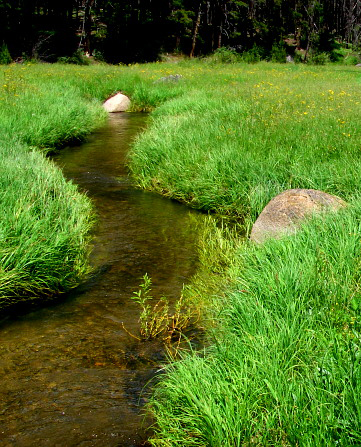
\includegraphics[scale=0.55]{scp/006.jpg}
\linebreak SCP-006
\end{center}
\end{figure}

\textbf{Special Containment Procedures:} Whereas the nature of SCP-006 does not warrant any extensive containment, a certain level of secrecy is necessary regarding the object's existence and properties, for obvious reasons. The following procedures are required not for personnel safety, but to deny or hide knowledge of SCP-006's effects from the personnel who interact with it.

1: All personnel interacting with SCP-006 in any physical way are required to wear modified class VI BNC suits. Before personnel are allowed to perform procedures, they must be briefed with Material SCP-006B or SCP-006C. SCP-006A Briefing is the correct one and is restricted to only those with O5 clearance. To assure personnel are wearing suits properly, they are to be submerged into a pool of water. Any air bubbles spotted signify a leak in the suit.

2: Procedures with SCP-006 are to be carried out under extreme surveillance. In case of contact with SCP-006, the commander in charge will announce procedure [EXPUNGED], which the personnel have been briefed to believe to mean high toxicity is present and they must evacuate.

3: Any procedure in which liquid is acquired from SCP-006 must be approved by three (3) O5 level personnel. The liquid is to be transferred in a Quad-Sealant Container and under armed guard.

4: If at any time personnel come into contact with SCP-006 or liquid from SCP-006, they are to be confined and terminated after sufficient studies are done. Due to the nature of SCP-006, the most effective termination method is incineration. (For full report, see file SCP006-TerO5)

\textbf{Description:} SCP-006 is a very small spring located 60 km west of Astrakhan. Due to political reasons, Foundation Command was aware of its existence since 18\censor{XX}, but unable to secure it until 1991. On the spot of the spring, a chemical factory has been constructed as a disguise, with the majority of laborers under Foundation and/or Russian control. The liquid emitted from the spring has been chemically identified as simple mineral water in 1902, but has the unusual property of "health".

Ingesting the liquid produces the following properties in human beings: the ability to regenerate DNA damaged by sufficient duplication, heightened excitement of cellular duplication, vastly improved abilities in the repair of damaged tissue, and a frightening increase in the effectiveness of the human immune system. Upon testing the liquid on animal subjects, hostile bacteria and viral agents were destroyed immediately. Many reptiles and birds were unaffected, while higher primates experienced the same benefits as humans.

\textbf{Addendum 1:} Permission for comparing samples of SCP-006 for similarity to SCP-500 has been requested by Dr. \censor{XXXXXX}-6
\toclesssection{SCP 007 - Abdominal Planet}
\addcontentsline{toc}{section}{SCP 007 - Abdominal Planet}
\fakebold{Item \#:} SCP-007

\fakebold{Object Class:} Euclid

\fakebold{Special Containment Procedures:} SCP-007 is to be contained in a sealed room measuring 10 m on each side. Room is to be furnished comfortably as a living area, along with whatever items are requested by \censor{XXXXXXXXXXXXXXX} (hereafter referred to as Subject), given that providing Subject with requested items would not compromise security. Subject is not to be allowed to leave the room, and is to be detained with force if necessary.

\fakebold{Description:} SCP-007 is located within a cavity in the abdomen of Subject. Subject is a Caucasian male, physically approximately 25 years of age (subject claims to be 28) and 176 cm in height. Most of Subject's abdomen (muscles, skin, and organs) is absent, though Subject does not appear to suffer because of this. Instead of normal flesh, a sphere composed of soil and water is present, though it does not actually come into contact with Subject's body at any point. The sphere appears to be in most respects a miniature near-duplicate of the Earth, approximately 60 cm in diameter, although continental alignment is not consistent with that of any alignment known in Earth's history. Sphere has its own weather patterns and negligible gravitational pull, in addition to microscopic organisms somewhat resembling those of modern-day Earth inhabiting it. Two intelligent species have been observed, though contact and communication with either has yet to be made. Technology levels of observed species must be checked at least once a week and, as of \censor{XX}/\censor{XXXX}, are approximately equal to that of 15th-Century Earth.

Subject claims to be named \censor{XXXXXXXXXXXXXXX}, but no records of such a person can be found. Subject does not require food or water, and while he has been observed consuming both, what happens to such substances after being swallowed is unknown. Subject is intelligent (IQ has been measured at 128) and amiable, and regards the planet in his abdomen as a minor curiosity about his body. Subject seems to experience no stress about his unusual condition. When questioned about planet's origins, Subject replied, "I just woke up one day, and there it was. I don't have any idea how it got there." Subject has provided a Social Security number and driver's license number and requested that they be checked against known records. When checked, it was discovered that neither had yet been allocated.

Dr. \censor{XXXXXXX} has a weekly chess game with Subject, during which Subject's mental health is evaluated. Dr. \censor{XXXXXXX} reports that Subject does not seem to mind the restricted living environment, and has yet to attempt to escape or show signs of violence or mental illness, though he has repeatedly requested a computer with an internet connection. It is recommended that this not be provided as it may be used to compromise security.
\toclesssection{SCP 008 - Zombie Plague}
\addcontentsline{toc}{section}{SCP 008 - Zombie Plague}
\begin{center}
$==$ LEVEL 4 CLEARANCE REQUIRED $==$\linebreak
Security Clearance Adequate: Access Authorized
\end{center}

\fakebold{Item \#:} SCP-008

\fakebold{Object Class:} Euclid

\begin{center}
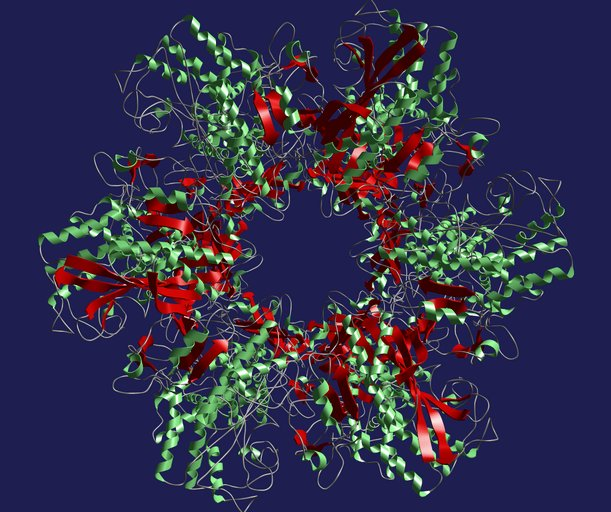
\includegraphics[scale=0.33]{scp/008.jpg}
\end{center}

\fakebold{Special Containment Procedures:} SCP-008 samples are extreme biological hazards and all related protocols apply. Incineration and irradiation measures will be deployed in the event of political or military action which may result in the facility being dismantled; a power failure; or zero communications from operatives or outside channels during any given eight (8)-hour period. The quarantine period for operatives leaving the facility is four (4) months. If a breach has occurred, incineration and irradiation measures shall be deployed. It should be the policy of all G2 sites to not prepare an evacuation procedure.

\fakebold{Description:} SCP-008 is a complex prion, samples of which are stored in each of the known G2 sites. Research into SCP-008 is highly classified and primarily aimed at preventing research which may lead to the synthesis of SCP-008 in the distant future. Traits of the SCP-008 prion include:
\begin{itemize}
\renewcommand{\labelitemi}{$\ast$}
\item 100\% infectiousness.
\item 100\% lethality.\newpage
\item Transmission through exposed mucous membranes and all bodily fluids.
\item Not airborne or waterborne.
\end{itemize}
Symptoms of infection with SCP-008 manifest no more than three hours after exposure, and include:
\begin{itemize}
\renewcommand{\labelitemi}{$\ast$}
\item Flu-like symptoms with high fever, plus severe dementia in later stages.
\item Coma onset approximately 20 hours after first symptoms appear and 12 hours after noticeable dementia. Coma onset will be considered onset of death.
\item A period of sporadic cellular necrosis occurs which comes to resemble gangrene. \item Surviving tissue assumes its original function and is highly resilient.
\item Red blood cells greatly increase oxygen storage capacity, resulting in slower blood flow and increased muscle endurance and strength.
\item Nervous and muscular systems are unaffected by total organ failure for several hours.
\item Metabolism may decrease to extremely low levels, allowing subject to survive for over 10 years without nutrition.
\item High blood viscosity results in negligible blood flow from gunshot, puncture, and slashing injuries.
\item Conditioned behavior, motor controls, and instinctive behavioral mechanisms are damaged, and cognitive abilities are severely retarded and erratic. Animals experience excessive brain necrosis and are inactive.
\item Subject can adapt to its damaged nervous systems but is limited to basic physical activities, including standing up, balancing on two legs, walking, biting, grabbing, and crawling. Subject will energetically move towards sights, sounds, and smells it associates with living humans. Subject will attempt to ingest living humans if physical contact is made.
\item Neutralizing fully-infected subjects requires significant cranial trauma.
\end{itemize}
There is strong evidence to suggest SCP-008 itself did not form naturally on Earth, since variants of similar complexity would have displaced much of the ecosystem. In 1959, a short collaborative effort with the USSR to locate G2 sites and eliminate SCP-008 was negotiated following their discovery. The status of SCP-008 in Russian custody since collaboration ended is unknown.

\fakebold{Addendum 008-1:} SCP-500 has been found to be able to completely cure SCP-008 even in the advanced stages of the disease.
\toclesssection{SCP 009 - Red Ice}
\addcontentsline{toc}{section}{SCP 009 - Red Ice}
\textbf{Item \#:} SCP-009

\textbf{Object Class:} Euclid

\begin{figure}[h]
\begin{center}
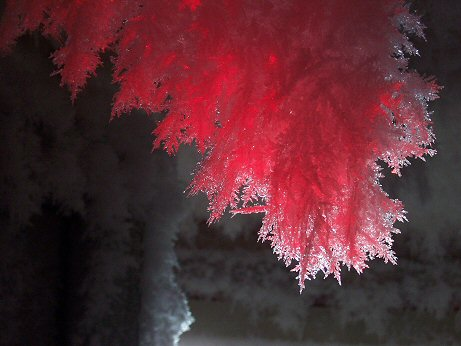
\includegraphics[scale=1.3]{scp/009.jpg}
\linebreak SCP-009 prior to recovery
\end{center}
\end{figure}


\textbf{Special Containment Procedures:} Subject is to be contained within a sealed storage tank of heat-resistant alloy with dimensions not less than 14m$^3$.

Under no circumstances should SCP-009 be exposed to temperatures in excess of 0°C when not undergoing testing, and no mundane liquids in a solid state (especially frozen water) shall be allowed within 30 meters of the subject's containment area. Subject's chamber is to be fitted with temperature sensors which shall be monitored at all times, and is to be kept refrigerated by no fewer than three (3) redundant cooling units. Any malfunction of sensors, or of coolant systems, is to be reported and repaired immediately.

If at any time the temperature in the containment area climbs above -5°C, the chamber is to be locked down immediately, and flooded with coolant until the temperature has been brought back down to between -30\degree C and -25\degree C. Atmosphere must be evacuated from the containment area when personnel are present within, and any water vapor present must be filtered and kept in the same conditions as detailed herein for no fewer than 24 hours. Any vapor displaying properties of SCP-009 is to be quarantined and added to the containment area as soon as possible.
\newpage
All personnel interacting with or observing the subject must wear full environmental protection suits. All personnel leaving the containment chamber must undergo dehydration of all gear, research materials, and other objects contacting SCP-009's chamber. If contamination is discovered, no material or personnel shall be permitted to exit, and a Level 2 lock-down of the containment area shall commence. Lethal force is authorized in cases of dire need, but all security forces are strongly advised to remain as far away from their targets as possible, to minimize the chance of contact with fluids contaminated by SCP-009.

\textbf{Description:} SCP-009 is approximately 3,700 liters of a substance which exhibits a number of unique properties. While small amounts of the substance, in all phases, are as colorless as mundane water, en masse it takes on a distinct deep red hue.

Its most notable property, however, is the fact that SCP-009's reaction to temperature extremes is exactly opposite that of standard H$_{2}$O: the subject assumes a liquid phase at temperatures between -100\degree C and 0\degree C, and converts into a solid state above those temperatures. At temperatures below -100\degree C, SCP-009 vaporizes into a gaseous phase similar to steam, though it still retains its red coloration when put under high pressure.

Examinations of the atomic structure of SCP-009 have proved inconclusive. Tests indicate that the subject is composed of the same combination of hydrogen and oxygen as normal water, leaving researchers to speculate that the source of the subject's abnormalities may be the atoms themselves. Dr. \censor{XXXXXX} has suggested that the subject may have originated in or been altered by another reality in which the laws of physics are inverted.

This theory may have some merit in light of SCP-009's marked ability to "assimilate" natural water into its mass. If placed in physical contact with any aqueous solution (be it ice, salt water, or water vapor in air), SCP-009 will "spread" and contaminate any H2O in said solution, causing it to exhibit the subject's properties. Though this capacity is present in all phases, it has been observed to progress most slowly (and thus be most containable) in the liquid phase.

If the subject comes in contact with any biological source of heat, it begins a runaway reaction in which the living organism's bodily fluids are rapidly converted to SCP-009 and promptly frozen by their own body heat (because of their generally high core temperatures, mammals are particularly susceptible). Because SCP-009 produces heat while freezing (at the same rate mundane ice consumes heat while melting), the process is self-perpetuating until all available moisture is converted, or until it is halted by external interference.
\newpage
Experiments on D-Class personnel have illustrated the process of conversion by the subject, which has been condensed down to a series of steps:

1. Initial Exposure: Subject is exposed to SCP-009, and it begins converting any water present on the exposed surface (usually skin) to exhibit its properties. Presence of mist, fog, snow, or other solid or vaporous water greatly accelerates this process.

2. Surface Conversion: A thin layer of frost forms on the exposed area as body heat and heat produced by SCP-009 raise its temperature above freezing. Progression to this step can take anywhere from five (5) minutes to one (1) hour, depending on victim's body temperature. At this stage, freezing has begun progressing through the initial layers of the epidermis and soon reaches live cells.

3. Deep Tissue Conversion: Exponential increase in temperature of SCP-009 causes expansion of ice crystals throughout the victim's body, resulting in widespread perforation of internal cell structure. Actual blood loss is minimal at this stage due to the crystals filling the puncture wounds, allowing subjects to remain alive and conscious for up to \censor{XX} hours.

4. [DATA EXPUNGED]

5. Death: Multiple organ failure and exsanguination via systemic crystallization.

Testing on D-Class personnel was discontinued as of\linebreak 4/23/20\censor{XX}.

\textbf{Addendum: Circumstances of Retrieval:} Subject was found in \censor{XXXX}, Alaska, on 11/05/19\censor{XX}. The Foundation got involved after reports were obtained from the native \censor{XXXX} Tribe, who came across the mangled bodies of a team of seal hunters which had apparently been ship-wrecked \censor{XX} kilometers from the village.

All victims were found encased in red ice. Cause of death recorded as internal bleeding. On victims whose features were sufficiently intact, expressions of panic and intense pain were observed. It is surmised that the low ambient temperatures in the area retarded the freezing process. This prolonged the time to total conversion by \censor{XX} hours, and allowed the victims to remain conscious until [DATA EXPUNGED].

\textbf{Addendum:} 12/16/20\censor{XX}

Super-cooling of SCP-009 for the purposes of experimentation is disallowed until further notice. Personnel are advised that liquid nitrogen is only to be used on the subject in controlled amounts, and only until temperatures have reached acceptable levels.

Related note: Possible application of SCP-009 in cold fusion research pending evaluation.
\toclesssection{SCP 010 - Collars of Control}
\addcontentsline{toc}{section}{SCP 010 - Collars of Control}
\fakebold{Item \#:} SCP-010

\fakebold{Object Class:} Safe

\fakebold{Special Containment Procedures:} The objects comprising SCP-010 are to be kept in numbered locked boxes in a high security facility. They are not to be worn except by test subjects.

SCP-010 are only to be removed from storage for testing.

\fakebold{Description:} SCP-010 consists of a series of six (6) apparently identical cast iron collars with numbered metal tags and one (1) remote control. The control is SCP-010-1. The collars are SCP-010-2 through 010-7. The collars contain intricate electronic components and are powered by small (5 mm diameter, 2 mm thick) 100 V batteries. These batteries are rechargeable.

The remote is a heavy black box resembling an old style hand-held radio transmitter/receiver with a primitive blue/white cathode ray screen and a series of more than 100 unlabeled buttons, as well as a frequency tuner. Through trial and error the frequencies of all six (6) currently found collars have been discovered. A label in Russian is stamped into the metal along with a logo consisting of workers building a pyramid. No official Russian corporation or government agency uses this logo or matches the words stamped into the metal.

Placing the collar around the neck of a person, and securing it, allows one to control their every movement with the remote. It is also capable of producing an adrenal response and activating or deactivating the sympathetic nervous system. The most abnormal feature of the collars is the effect they have on the body morphology. They allow the user of the remote to reconfigure the shape of the victim to an extent that is apparently only limited by the knowledge of the programming language of the remote.

\fakebold{Addendum 010-1:} History

SCP-010 was discovered in the basement of a lone man in the Midwestern United States after a local disappearance was connected to him. When the police raided the man's house they found SCP-010 as well as several dead bodies. One of the bodies was identified to be the man. The others were several other missing persons. Cause of death seemed to be mass suicide; however, there were signs of significant struggle first.

\fakebold{Addendum 010-2:} Disassemble experiment

Test 1: SCP-010-2 taken apart piecewise, the parts labeled and several photographs taken, then reassembled.
Result: After reassembly SCP-010-2 continues to function.

Test 2: SCP-010-8 constructed identically to SCP-010-2 but with the closest approximations available to the unreplicable components.
Result: SCP-010-8 fails to function.

Test 3: Unreplicable components from SCP-010-2 placed into proper locations on SCP-010-8.
Result: SCP-010-2 ceases functioning with removal of components. SCP-010-8 begins functioning.

Test 4: Components returned to SCP-010-2. Replicable components in SCP-010-2 replaced randomly with replicas
Result: SCP-010-2 begins functioning with return of components. Changing replicable components for replicas does not significantly reduce functionality. Replacement of a damaged transistor decreased time from transmission to effect of SCP-010-2 response to commands entered in the remote by 12%.

\fakebold{Addendum 010-3:}

SCP-010 has been demonstrated to work more effectively in creating unskilled labor than for any other task. The logo is apt. -- \textasciitilde Dr. \censor{XXXXX}
\toclesssection{SCP 011 - Sentient Civil War Memorial Statue}
\addcontentsline{toc}{section}{SCP 011 - Sentient Civil War Memorial Statue}

\textbf{Item \#:} SCP-011

\textbf{Object Class:} Safe

\begin{figure}[h]
\begin{center}
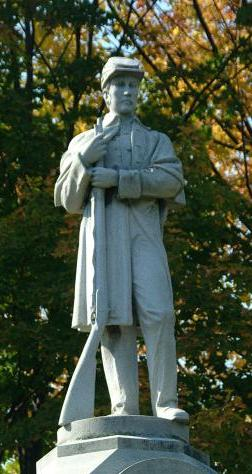
\includegraphics[scale=0.6]{scp/011.jpg}
\linebreak SCP-011
\end{center}
\end{figure}

\textbf{Special Containment Procedures:} Item SCP-011 and the area surrounding it are to be cleaned once every day. For safety purposes, cleaning should start at least 30 minutes after sundown. Cleaning should always be performed by at least two (2) personnel, who are also advised to note anything unusual about the item or the debris cleaned up. In a situation where the item cannot be cleaned for more than two (2) days, local residents must be contacted and instructed not to approach the item.

\lb Containment procedures nullified 2004\rb

\textbf{Description:} SCP-011 is a Civil War memorial statue located in Woodstock, Vermont. The statue is the image of a young male soldier holding a musket at his side, and is carved out of granite quarried within the area. Occasionally, SCP-011 has been observed lifting its musket to the sky to fire at birds which attempt to land or defecate on it. Reports detail that its movements produce soft grinding sounds but do not cause it any structural failure. Oddly, the gunfire is very similar to that of a standard firearm, despite observations that the item only loads granite bullets and granite powder into the musket (which is also unharmed by the firing). In spite of its efforts, some fecal matter does manage to strike SCP-011, and it has reportedly become distressed when it has had a large amount of feces on it, on some rare occasions even firing at humans.

\textbf{Addendum:} Those assigned to maintain SCP-011 are to see document \#011-1 for instructions.

\begin{leftbar}
\textbf{Document \#011-1: Maintenance Brief}

\lb Document archived 2004 - accessible to personnel with security clearance 2/011 or higher\rb

Additional Information: SCP-011's seeming sentience has increased since the first report of activity in 1995. As of 2004, the item's containment procedures have been dropped but it remains under constant observation. Recorded below are landmark events in its activity.

Timeline:
\begin{flushleft}
3.12.1995 - Woodstock resident reports the statue's eyes moving, first sign of activity\linebreak
9.30.1995 - Statue shoots musket for the first time\linebreak
10.9.1995 - Statue begins shooting birds from the sky\linebreak
1.25.1996 - Registration as SCP-011, containment procedures begin\linebreak
4.14.1997 - SCP-011 observed moving casually and looking around\linebreak
5.3.2000 - After caretaker \censor{XXXX} \censor{XXXXXXXX} jokingly shouts "Good shot!" to SCP-011, the item replies, "Thank you," in a reportedly very human voice, first speech from statue\linebreak
10.22.2001 - SCP-011 has conversation with caretaker \censor{XXXXXXXXX} \censor{XXXXX}
2001 - Shooting of birds stops
2.6.2002 - At the imploring of \censor{XXXXXXXXX} \censor{XXXXX}, SCP-011 steps down from its pedestal
2003-2004 - SCP-011 reaches a human level of self-awareness
11.10.2004 - Containment procedures dropped, custody of SCP-011 transferred to \censor{XXXXXXXXX} \censor{XXXXX}
5.17.2005 - \censor{XXXXXXXXX} \censor{XXXXX} reports that SCP-011 is romantically attracted to her
8.29.2006 - Most recent psych test reports an IQ of 133
\end{flushleft}
\end{leftbar}
\toclesssection{SCP 012 - A Bad Composition}
\addcontentsline{toc}{section}{SCP 012 - A Bad Composition}

\fakebold{Item \#:} SCP-012

\fakebold{Object Class:} Euclid

\fakebold{Special Containment Procedures:} SCP-012 is to be kept in a darkened room at all times. If the object is exposed to light or seen by personnel using a light frequency other than infrared, remove personnel for mental health screening and immediate physical. Object is to be encased in an iron-shielded box, suspended from the ceiling with a minimum clearance of 2.5 m (8 ft) from the floor, walls, and any openings.

\fakebold{Description:} SCP-012 was retrieved by Archaeologist K.M. Sandoval during the excavation of a northern Italian tomb destroyed in a recent storm. The object, a piece of handwritten musical score entitled "On Mount Golgotha", part of a larger set of sheet music, appears to be incomplete. The red/black ink, first thought to be some form of berry or natural dye ink, was later found to be human blood from multiple subjects. The first personnel to locate the sheet (Site 19 Special Salvage) had two (2) members descend into insanity, attempting to use their own blood to finish the composition, ultimately resulting in massive blood loss and internal trauma.

Following initial investigations, multiple test subjects were allowed access to the score. In every case, the subjects mutilated themselves in order to use their own blood to finish the piece, resulting in subsequent symptoms of psychosis and massive trauma. Those subjects who managed to finish a section of the piece immediately committed suicide, declaring the piece to be "impossible to complete". Attempts to perform the music have resulted in a disagreeable cacophony, with each instrumental part having no correlation or harmony with the other instruments.
\toclesssection{SCP 013 - Blue Lady Cigarettes}
\addcontentsline{toc}{section}{SCP 013 - Blue Lady Cigarettes}

\fakebold{Item \#:} SCP-013

\fakebold{Object Class:} Safe

\begin{figure}[h]
\begin{center}

\includegraphics[scale=1.4]{scp/013.jpg}
\linebreak SCP-013
\end{center}
\end{figure}

\fakebold{Special Containment Procedures:} SCP-013 are to be kept in a Secure Storage Vault at Site-66. Exposed subjects are to be monitored for differences between their symptoms. Any differences between exposed subjects are to be logged and studied. Exposed subjects are to be interviewed daily.

\fakebold{Description:} SCP-013 is the collective designation of 242 cigarettes which display similar anomalies. The most common external detail between instances is the presence of the words “Blue Lady” hand-written on each cigarette in blue ink.

Subjects who consume the contents of SCP-013 through inhalation will begin to perceive themselves as a specific unidentified woman. Subjects have described the woman to be aged between 25 and 35 years old, standing approximately 1.6 metres tall with an estimated weight of between 50 and 55 kg. Additional recurring details include cropped dark hair, blue eyes, and bright blue lipstick.

Immediately after consuming an instance of SCP-013, subjects will perceive all of their own reflections as those of the woman. Over the following weeks, subjects will gradually begin to perceive themselves as having the features of the woman, and will gradually perceive their bodies changing to reflect her appearance. All changes are entirely mental; the subject’s body does not change outwardly, only their perception of themselves. These alterations are permanent, and cannot be reversed.

SCP-013 was discovered after the suicide of an Ian Miles, packed in a large cardboard crate in his apartment. A cursory search of the apartment uncovered several hundred sketches of a figure strongly resembling the one perceived while under 013's effect. Miles' body had been found sitting at a desk, dead of a massive overdose and draped over a handwritten note, transcribed below.

During the investigation of Miles' apartment, one civilian investigator became affected by 013's effect. An embedded Agent soon contacted the nearest Site; the subject, the artifact, and related evidence were extracted and contained.

\fakebold{Addendum:} Below is the note which was acquired along with SCP-013.

\begin{boxedminipage}{\textwidth}
\begin{flushleft}

I don't know what happened to me. I see her everywhere.\linebreak

I know I should know who she is but I can't remember. I love her but I don't know who she is. She's so beautiful but \sout{I want} can't remember. I used to know her but i don't know any more. \sout{where did you go} I miss you\linebreak

she left me her favorite flavor
\end{flushleft}
\end{boxedminipage}
\toclesssection{SCP 014 - The Concrete Man}
\addcontentsline{toc}{section}{SCP 014 - The Concrete Man}

\fakebold{Item \#:} SCP-014

\fakebold{Object Class:} Safe

\begin{figure}[h]
\begin{center}
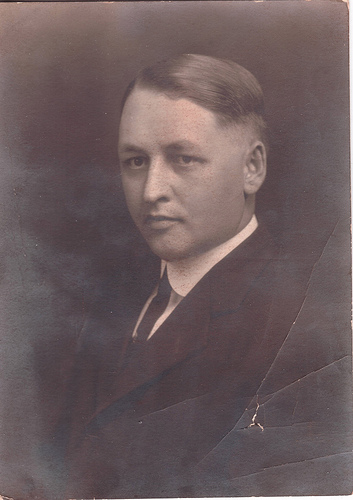
\includegraphics[scale=4]{scp/014.jpg}
\linebreak SCP-014 prior to initial confinement
\end{center}
\end{figure}

\fakebold{Special Containment Procedures:} SCP-014 is to be kept in Site-\censor{XX}, in a chair with arms, preferably facing a window. Music should be supplied on a regular basis, preferably constantly. This music should not include pieces originating after 1937. A security camera should be present in SCP-014's room.

\fakebold{Description:} SCP-014 is a Caucasian male, appearing to be approximately 30 years of age, with black hair, brown eyes, and a somewhat round face. Records indicate his name to be Robert Chetford, confined in 1915 to the Norwich Asylum in Connecticut for delusional insanity, claiming that he had been cursed to live forever, and was slowly turning into concrete in consequence. The asylum closed in 1937, and the patients were transferred to various other facilities. SCP-014 came to Foundation attention in 19\censor{XX}, from rumours of a patient who seemed to be entirely immobile and showed no signs of aging. Further investigation determined that acquisition was warranted.
\newpage
SCP-014 is to all outward appearances a normal man, but he does not appear to age, and shows no signs of possessing a metabolism. He does not eat, drink, perspire, or in any other way demonstrate life functions. He breathes only to speak, and apart from his eyes and vocal apparatus, is to all appearances utterly immobile. He has never shown any evidence of pressure ulcers despite his position not having varied for several decades; neither do his muscles appear atrophied. He can converse normally, but shows little knowledge of or interest in events since his confinement.

\fakebold{Addendum:}\linebreak
Note: Frankly, were I to interview this man without knowing his history, I'd think he was a perfectly sane and well-adjusted individual who happens to be quadriplegic. As it is, I have to conclude that he's the ultimate proof of the idea that the mind rules the body. He thinks he's concrete, and will live forever, and so he's as close to both as he can be. Somehow. Dr. \censor{XXXXX}
\toclesssection{SCP 015 - Pipe Nightmare}
\addcontentsline{toc}{section}{SCP 015 - Pipe Nightmare}

\fakebold{Item \#:} SCP-015

\fakebold{Object Class:} Euclid

\begin{figure}[h]
\begin{center}
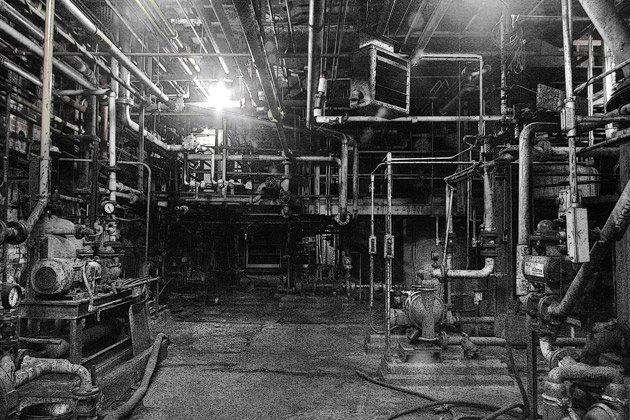
\includegraphics[scale=0.4]{scp/015.jpg}
\linebreak SCP-015
\end{center}
\end{figure}

\fakebold{Special Containment Procedures:} SCP-015 is impossible to move, and is contained on-site. A gap of at least 2 m (6 ft) needs to be maintained around the entire structure containing SCP-015 at all times, and no structures of any kind are to make contact with SCP-015's current containment structure. Exploration is permissible, but only in teams of three (3) with full safety lines and GPS tracking. Any protrusions from SCP-015 must be capped and sealed immediately, with the new site recorded and logged.

No aggressive action is to be made within SCP-015. No hand or power tools are allowed anywhere inside SCP-015. No repairs or maintenance are to be made anywhere on SCP-015.

\fakebold{Description:} SCP-015 is a mass of pipes, vents, boilers and other various plumbing apparatus completely filling a warehouse in \censor{XXXXXXX}. The pipes appear to grow when not under observation, attempting to connect to nearby structures via sewer systems and underground plumbing. SCP-015 contains, at current estimate, over 190 kilometers (120 miles) of pipes, ranging in diameter from 2.5 cm to over 1 m. Some pipes appear new, while others are rusted and leaking. Pipes have been reported as being made of bone, wood, steel, pressed ash, human flesh, glass, and granite. No pipes composed of lead, PVC plastic, copper, or any other traditional material for the production of pipes have been found.

SCP-015 reacts to tools and aggression. Any personnel acting violently, carrying tools, or attempting to damage or repair SCP-015 in any way, will trigger a reaction. Any pipes near the subject will burst, spraying on the subject for several seconds before the flow suddenly stops. Pipes have been reported containing oil, mercury, rats, a species of insect not yet identified, ground glass, sea water, entrails, and molten iron. Pipes will continue to burst around subject until death or retreat.

SCP-015 was cut back to its current structure after attaching to 11 other structures in the area. Currently, 11 personnel have been killed, and 20 more are still missing. Reports have been made of banging and screaming coming from within SCP-015.
\toclesssection{SCP 016 - Sentient Micro-Organism}
\addcontentsline{toc}{section}{SCP 016 - Sentient Micro-Organism}

\fakebold{Item \#:} SCP-016

\fakebold{Object Class:} Keter

\fakebold{Special Containment Procedures:} SCP-016 is to remain within the confines of a five by five by five (5x5x5) meter room at all times, maintained at a temperature not to exceed zero (0) degrees Celsius. SCP-016 itself is to remain in the petri dish in the containment cube at all times unless directed otherwise by Level 4 or O5 personnel. Full documentation of experimentation with SCP-016 must be submitted before and after samples and duplicates of SCP-016 may be taken. Failure to follow these procedures will result in termination or reassignment as Class-D Personnel. Only authorized personnel may be permitted to obtain samples of and experiment with SCP-016 under BC-L5 containment conditions.

If an outbreak does occur despite following the aforementioned procedures, directive base personnel are to implement a Code Sigma lockdown and containment plan. Infected personnel are to be terminated on site by security forces wearing standard Mission Oriented Protective Posture (MOPP) anti-biological and anti-chemical equipment. Should the infection not be contained after 48 hours, the on-site nuclear device is to be detonated. Remaining personnel are not to be evacuated under any circumstances.

SCP-016 has been shown to survive for up to six (6) hours in blood, and up to several minutes in air. High intensity ultraviolet light and high concentrations of chlorine bleach have been demonstrated to be effective in sterilizing nonorganic materials.

\fakebold{Description:} SCP-016 is a blood-borne pathogen recovered from a mine worker in \censor{XXXXX} who injured himself while working in a deep coal seam. Said wound became contaminated with coal dust from the mine, possibly infecting the worker with dormant spores. Over the next several days, SCP-016 proceeded to infect the remaining employees at the mining camp, as well as the CDC crisis team dispatched to deal with the epidemic. Foundation personnel then took over the investigation and terminated all affected personnel. Patient Zero was brought into captivity, and the mine shaft was collapsed by explosive device.

SCP-016 has an incubation period ranging from 24 hours to two (2) years, depending on the presence and number of other human hosts in the area. First symptoms resemble the common cold, and include itchy eyes, runny nose, coughing, and bodily aches. Phase two begins in 48 hours, and consists of a controlled form of hemorrhagic fever, as the organism causes a small amount of blood to become aspirated in the lungs, creating an aerosol effect. During phase three, the host "crashes and bleeds out," bleeding profusely from every bodily orifice, including the nose, tear ducts, anus, skin pores, mouth, urethra, and (in case of females) vagina. Blood pressure skyrockets during the final stage: hosts have been observed projectile vomiting blood to distances of over five (5) meters. Should the host survive this near-total exsanguination, the pathogen will become dormant once more, returning to incubation phase.

What distinguishes SCP-016 from other strains of hemorrhagic fever such as Ebola and Marburg is its unusual response to high stress. Should the subject undergo a high-stress situation (such as a life-threatening crisis), the organism will mutate into a DNA retrovirus, changing its survival tactic from rapid reproduction to the rewriting of the host's DNA and stimulation of rapid cell division. Major physiological changes occur within the first 24 hours, with complete bodily reconstruction occurring within two (2) weeks time. Most hosts do not survive the process due to the heavy demands made on the body.

An interesting side effect of the transformation is an increased aggressive urge. It is believed that this may be an attempt to maximize the spread of the virus in a manner similar to rabies. On another note, subjects who undergo bodily transformation no longer appear to exhibit SCP-016's hemorrhagic properties: however, subjects infected by transformed hosts will still undergo the normal SCP-016 infection process.
\newpage
\begin{flushleft}
\fakebold{Addendum: Experiment Log of SCP-016's Transformative Properties}
\end{flushleft}

\begin{itemize}
\renewcommand{\labelitemi}{$\ast$}
\item Subject D-016-1: D-Class personnel infected by SCP-016. Upon first showing symptoms, subject's quarters were slowly flooded with water over a 24 hour period. SCP-016 mutated into teratomorphic state, transforming subject's lungs into gills. Subject survived for two (2) more weeks as SCP-016 transformed its limbs into fins, caused its eyes to atrophy, and enhanced its sense of hearing into a cetacean-type echolocation ability. Subject was terminated by draining all water from its quarters, causing it to asphyxiate: body was subsequently cremated without autopsy.
\item Subject D-016-2: D-Class personnel infected by SCP-016. Upon first showing symptoms, subject's quarters were slowly flooded with water over a 24 hour period. SCP-016 mutated into teratomorphic state, causing subject to undergo rapid muscular growth and increased bone growth on knuckles. Subject then attempted to escape from confinement by punching through the reinforced steel door. Subject was not successful and died by drowning.
\end{itemize}
\textsl{Note: Same situation, two different responses. Interesting. - Dr. \censor{XXXXXXXX}}

\begin{itemize}
\renewcommand{\labelitemi}{$\ast$}
\item Subject D-016-3: D-Class personnel infected by SCP-016: subject was previously a chemical engineer who poisoned his wife upon discovering her adultery. Upon first showing symptoms, subject's quarters were slowly flooded with water over a 24 hour period. SCP-016 mutated into teratomorphic state, causing subject to grow an unusual organ on his chest, consisting of a chamber and two (2) separate tubes. Organ continued to take in water and swell in size, until Foundation personnel, realizing what SCP-016 may be attempting, terminated the subject by gunshot. Organ was found to contain several gas sacs filled with acetylene gas and oxygen.
\newpage
\item Subject D-016-4: D-Class personnel infected by SCP-016. Subject was told to concentrate on forming wings. No stress was applied. SCP-016 did not mutate into teratomorphic state. Subject died of exsanguination during Phase 3.
\item Subject D-016-5: D-Class personnel infected by SCP-016. Subject was told to concentrate on forming wings and placed in an acrylic box suspended 305 m (1000 ft) above a mine shaft. A timer was placed outside the box which subject was told indicated the time to release. SCP-016 mutated into teratomorphic state, causing subject to grow a tentacle-like organ on his left wrist similar to a spider's spinnerets: subject extended said organ through one of the box's air holes and extruded a strong, silk-like substance, which it then used to secure the box to the cable. Subject was terminated when the countdown reached zero and the bomb detonated.
\end{itemize}
\toclesssection{SCP 017 - Shadow Person}
\addcontentsline{toc}{section}{SCP 017 - Shadow Person}

\fakebold{Item \#:} SCP-017

\fakebold{Object Class:} Keter

\begin{figure}[h]
\begin{center}
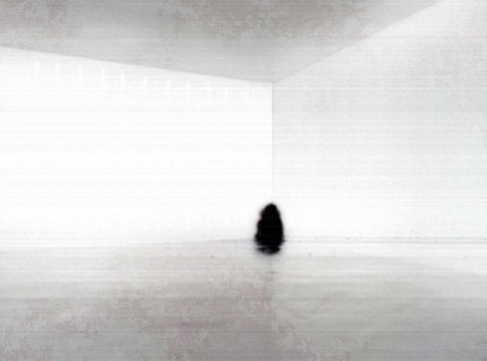
\includegraphics[scale=0.5]{scp/017.jpg}
\linebreak File footage of SCP-017
\end{center}
\end{figure}

\textbf{Special Containment Procedures:} SCP-017 is contained in an acrylic glass cage, 100 cm by 50 cm by 50 cm, centrally suspended in a concrete room measuring 6 m by 6 m by 4 m. Attached to the walls, ceiling, and floor of the room are high-intensity arc lamp spotlights pointed directly at the acrylic cage, to ensure that SCP-017 is constantly exposed to light from every angle. Personnel assigned to the SCP-017 control room are to monitor the functionality of the spotlights and the emergency generator system and call for maintenance immediately upon knowledge of a burnt-out lamp or an issue with the generator.

The only circumstance under which personnel are allowed entrance is to replace lamps. Personnel entering the room are required to wear the designated full-body reflective suits, and must be cautioned not to step in front of functional spotlights.

\textbf{Description:} SCP-017 is a humanoid figure approximately 80 centimeters in height, anatomically similar to a small child, but with no discernible identifying features. SCP-017 seems composed of a shadowy, smoke-like shroud. No attempt to find any object beneath the shroud has been successful, but the possibility has not been ruled out.

SCP-017's reaction to shadows cast upon it is immediate and swift. SCP-017 leaps at the object casting the shadow and completely encloses it in its shroud, whereupon it returns to its normal size, leaving no trace of the object behind.

\textbf{Additional Notes:} Personnel with BETA clearance or higher should see also document \#017-1.
\toclesssection{SCP 018 - Super Ball}
\addcontentsline{toc}{section}{SCP 018 - Super Ball}

\textbf{Item \#:} SCP-018

\textbf{Object Class:} Euclid

\begin{figure}[h]
\begin{center}

\includegraphics[scale=1.3]{scp/018.jpg}
\linebreak SCP-018
\end{center}
\end{figure}

\textbf{Special Containment Procedures:} SCP-018 is to be contained in the specialty metal restraint inside of a 1 m by 1 m by 1 m sealed box lined with heavy synthetic padding. The sealed box is then submerged in the center of the 10 m by 10 m by 10 m polyethylene holding tank. If SCP-018 is to break free from the holding box, the polyethylene-based 'goo' will slow down kinetic activity enough for proper retrieval by containment personnel. Personnel entering SCP-018's holding chamber are to wear specialized plating (found inside of SCP-018 Observation), and a breathing apparatus before being lowered into the polyethylene tank. If SCP-018 is loose outside of the polyethylene tank, personnel are advised to secure themselves in a separate room and close doorways or hatches to isolate SCP-018 until containment teams arrive.

\textbf{Description:} SCP-018 has the appearance of a Super Ball made by the Wham-O company in 1969. It is six (6) centimeters in diameter and coloured red. Found when the \censor{XXXXXXXXXX} company was hired to clean out a warehouse that had Wham-O merchandise in it, SCP-018 was noted to be able to bounce with extreme height. At first thought to be a pleasant child's toy, SCP-018 was able to bounce with over two hundred percent (200\%) efficiency (that is, if dropped one (1) meter, it would bounce two (2), then four (4), then eight (8), then sixteen (16)). The ball soon became a dangerous projectile, reaching speeds estimated at over 100 km/h and damaging property and injuring five (5) in the city of \censor{XXXXXXXXXXXXX}. It came to a rest after several days in the nearby lake of \censor{XXXXXXXX}, and was retrieved by SCP personnel. Due to the speed of the object, and the total surprise by its victims, no cover-up story was required or initiated.

\textbf{Document \#018-04:} Message to O5-\censor{X}

\textsl{\censor{XXXXXXXXX}, I hope everything is well. The reason I write to you is because I believe I have found a more effective method for retrieving new or escaped SCP objects. Yes, I realize we haven't had any progress in reverse engineering whatever allows this thing to defy the laws of thermodynamics, but we have come up with a very effective method for integrating one of those new SCP-A5 Armor suits with this. Just hear me out, we implant it into the bottom of a boot, rig up a little bit of a mechanical device, and ta-da, the suit is now capable of jumping well over a building. Also, if the wearer has their foot against something they want dead, well, lets just say it delivers a helluva kick. All I need is permission to modify one of the pre-existing SCP-A5 suits, and you'll be able to actually capture \censor{XXXXXXXXXXXX}, plus any other escaped SCP objects. Trust me, when have I let you down in the past?}

-Dr. \censor{XXXXXXXXXX}

\textbf{Document \#018-06:} Letter to Dr. \censor{XXXXXXXXX}
\textsl{\begin{flushleft}Dr. \censor{XXXXXXXXX},\end{flushleft}
Upon assignment, Agent \censor{XXXXXX} was issued your modified SCP-A5 armor in retrieving SCP-\censor{XXX}, and the results are mixed. Agent \censor{XXXXXX} was able to place the \censor{XXXXXXXXXX} collar onto SCP-\censor{XXX}, chase it through the Amazon, and restrain it by dismemberment. However, due to a malfunction of your 'little mechanical device', he was launched almost a mile into the air and suffered two broken legs, seven broken ribs, a missing arm, and a skull fracture upon hitting the water of Lake \censor{XXXXXXXXXXX} on the way back down. You will fix that before I authorize your armor for common use.}

\textbf{Document \#018-11:} Message to O5-\censor{X}

\textsl{\censor{XXXXXXXXX}, don't worry, it's fixed. But, I have some more ideas. If I can be granted the use of some water from SCP-006, SCP-\censor{XXX}, and possibly SCP-\censor{XXX}, I can deliver you a set of SCP-A5 armor and an agent that can capture any, if not all, rogue or unattained SCPs. All I'm waiting on is your approval.}
\toclesssection{SCP 019 - The Monster Pot}
\addcontentsline{toc}{section}{SCP 019 - The Monster Pot}

\textbf{Item \#:} SCP-019

\textbf{Object Class:} Keter

\begin{figure}[h]
\begin{center}
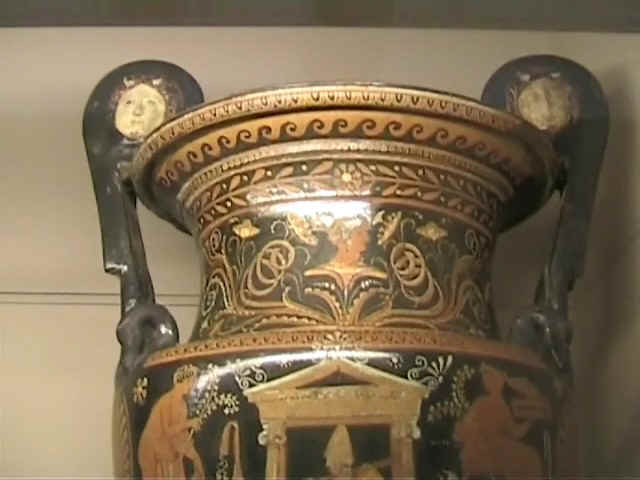
\includegraphics[scale=0.5]{scp/019a.jpg}
\linebreak SCP-019
\end{center}
\end{figure}

\textbf{Special Containment Procedures:} SCP-019 is to be placed on a wide grate in a 3 m x 3 m x 4 m room made of reinforced concrete, installed with an incinerator. Room is to be kept at zero (0) degrees Celsius when incinerator is not activated. An observation chamber separated by a plate glass window is to be used for constant observation of SCP-019, and if/when specimens of SCP-019-2 are noticed, the incinerator is to be activated. In case of an outbreak of SCP-019-2, ordinary firearms are successful in terminating individual specimens, although in the case of a swarm outbreak, flamethrowers may be more effective. SCP-019 should be kept in a vertical position at all times.

\textbf{Description:} SCP-019 appears to be a very large ceramic vase, 1.8 m in diameter at the mouth and 2.4 m high. Style and decoration indicate it was created in Classical Greece, although conclusive dating is impossible, as the surface is entirely unbreakable by any known means. If a successful method is discovered, SCP-019 is to be destroyed with prejudice.

Periodically, entities emerge from SCP-019. Collectively, these are known as SCP-019-2. The entities vary in many aspects, but tend to be small, vaguely humanoid (though they may have animaloid features), and extremely hostile. They often choose to attack with teeth or claws. Although fairly delicate (also, surprisingly, flammable), they are reasonably strong and pose a considerable threat in large numbers.

\begin{figure}[h]
\begin{center}

\includegraphics[scale=0.55]{scp/019b.jpg}
\linebreak SCP-019-2 specimen
\end{center}
\end{figure}

When kept at zero (0) degrees Celsius and totally at rest, entities will emerge from SCP-019 at a rate of approximately one (1) entity per hour. The following traits are known to affect SCP-019-2's manifestation rate:
\begin{itemize}
\renewcommand{\labelitemi}{$\ast$}
\item Movement of SCP-019
\item Threat to SCP-019
\item Extreme temperature in either direction
\item Sudden shift in surrounding environment in general
\item Introduction of objects or organisms to the inside of SCP-019 (known to cause a “flood” reaction)
\end{itemize}
Traits that may or may not influence SCP-019-2's manifestation rate:
\begin{itemize}
\renewcommand{\labelitemi}{$\ast$}
\item Presence of human life near SCP-019
\item Current weather patterns
\item Specific individuals near SCP-019 (some individuals seem to affect SCP-019-2's emergence rate more drastically than others)
\end{itemize}
In addition, tipping or tilting SCP-019 will create a reaction as though it was previously “filled” with SCP-019-2 specimens, although viewers looking into SCP-019 from above will merely note a dark hole. Due to the production rates of SCP-019-2 when the object is disturbed, measurement of the internal cavity is difficult, but it is suspected to be inconsistent with outside measurements.

\textbf{Addendum:} Document SCP-019-2-A
SCP-019-2 notes, as maintained by Doctor Light and Doctor Vaux

\censor{XX}/\censor{XX}/\censor{XXXX}\linebreak
SCP-019-2 specimen was removed from containment chamber and kept in reinforced pen, provided with water and live chickens as food. Specimen made quiet, continuous, garbled vocalizations, determined to be phonetically similar to Ancient Hellenic languages. Although it is unknown why this is, specimens are still thought to be no more intelligent than animals.

The specimen only lived for under 48 hours, and a dissection revealed anatomy consistent on a cellular level with normal biology, but with an extremely unstable musculoskeletal structure. Other notable anomalies included an unstable respiratory system, next to no digestive tract, and virtually no other internal organs. All other captured specimens have followed similar patterns of behavior and demise.

Note: It appears that SCP-019-2 specimens were not intended to live for meaningful amounts of time outside of SCP-019. - Dr. Vaux

\censor{XX}/\censor{XX}/\censor{XXXX}\linebreak
Containment unit was slightly damaged following prolonged exposure to SCP-019-2 specimen, missed by the monitoring team because of partial transparency. This has not been noted in SCP-019-2 before. Monitoring teams will continue to report further anomalies.

\censor{XX}/\censor{XX}/\censor{XXXX}\linebreak
Monitoring teams report some specimens of SCP-019-2 now appear to be significantly more resistant to incineration than others. It is hypothesized that this is a defense mechanism on the part of SCP-019.

\censor{XX}/\censor{XX}/\censor{XXXX}\linebreak
Most specimens of SCP-019-2 are now all but entirely resistant to the effects of the incinerator. Use of acid bath instead of incinerator is being considered. “Evolution” of SCP-019-2 is being studied, and may be evidence of sentience in SCP-019-2.
\toclesssection{SCP 020 - Unseen Mold}
\addcontentsline{toc}{section}{SCP 020 - Unseen Mold}

\textbf{Item \#:} SCP-020

\textbf{Object Class:} Keter

\begin{figure}[h]
\begin{center}
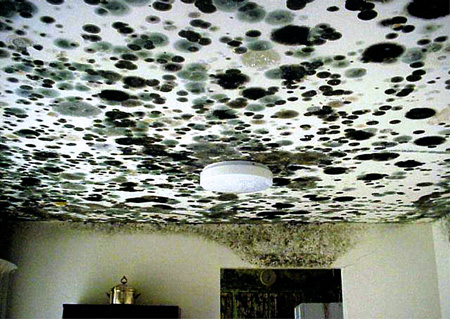
\includegraphics[scale=0.6]{scp/020a.jpg}
\linebreak SCP-020 growths in a civilian residence.
\end{center}
\end{figure}

\textbf{Special Containment Procedures:} Samples of SCP-020 are kept in a hermetically sealed cylindrical cultivation chamber measuring 1 m in diameter and 1 m high. This chamber is located inside a sealed containment room, accessible only via airlock. Nutrients are administered via automated robotic systems, as the cultivation chamber must remain sealed at all times.

Hermetically sealed video surveillance cameras are installed within the containment room, and must be checked daily for integrity. Any personnel entering the containment room must undergo a full anti-fungal disinfection procedure upon exiting.

\textbf{Description:} SCP-020 is a fast-spreading fungal organism that is capable of affecting the senses and behavior of living creatures, including humans. Samples of SCP-020 exhibit an unknown effect that renders them effectively invisible to direct observation, even when under a microscope. SCP-020 is only visible to humans when viewed through photographic or video surveillance.
\newpage
Once SCP-020 forms a colony, usually within a human residence, it will produce spores that affect the behavior of humans around it. Affected subjects will increase the heat and humidity within their homes to create an environment more suitable to the growth of SCP-020. Affected subjects also become more sociable in many cases, and often invite acquaintances to their homes to further spread the organism. As the spores and mold colonies are invisible to affected subjects, the mold may sometimes grow directly on living subjects.

\begin{figure}[h]
\begin{center}
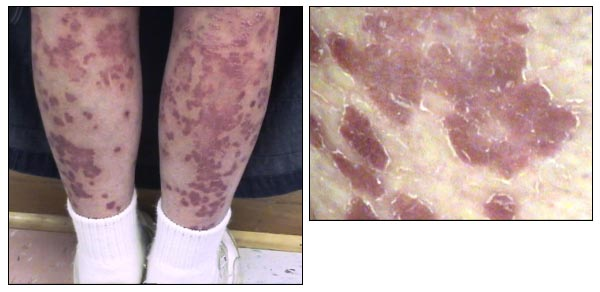
\includegraphics[scale=0.5]{scp/020b.jpg}
\linebreak A civilian infected with SCP-020 colonies.
\end{center}
\end{figure}

As the spores and colonies within a home approach critical concentration, the health of affected human subjects will rapidly deteriorate, resulting in death. Further spread of the mold may occur as the bodies of any deceased subjects are encountered by emergency responders and health care agents, as well as transportation of the bodies to local morgues.

SCP-020 was first encountered in \expunged, where an undercover SCP agent noted dramatic personality changes in personnel working at the local hospital. Upon investigation by a containment team, it was discovered that almost \censor{XXX} civilians had been infected, as well as a majority of the town. The civilian population was terminated, and the town incinerated under cover of a local flash forest fire.

To date, over 12 outbreaks of SCP-020 have been reported. Investigations are currently underway to determine the source of these outbreaks and possible preventative measures.

\textbf{Addendum 020-01:} Excerpts from the audio/video mission recorders of Mobile Task Force \expunged \ during the initial containment of SCP-020 at \expunged.

\begin{boxedminipage}{\textwidth}
\begin{flushleft}

\textbf{T2-Lead:} Team Two moving to the red house.\linebreak
\textbf{T2-COM:} Copy, UAV One is picking up one heat signature.\linebreak

...\linebreak

\textbf{T2-Lead:} Team Two in place, ready to br- \lb Expletive\rb!\linebreak
\textbf{T2-2:} The door's opening!\linebreak

\textsl{At this point, a civilian woman appeared in the doorway, holding a kitchen knife. Video surveillance showed that nearly two-thirds of her face was covered by mold growths.}\linebreak

\textbf{Civilian Woman:} Well… hello there, gentlemen… care to take a breather inside?\linebreak
\textbf{T2-Lead:} On the ground! Drop the weapon!\linebreak
\textbf{Civilian Woman:} Don't be silly! Come on in and… stay a while…\linebreak
\textbf{T2-Lead:} Stop where you are! DROP THE WEAPON!\linebreak
\textbf{Civilian Woman:} We... we just want to have some guests... please... come in...\linebreak
\textbf{T2-2:} Drop the \lb Expletive\rb \ weapon!\linebreak

\textsl{It is assumed that at this point, the infected civilian noticed T2-4 carrying a primed incendiary weapon, and lunged forward at the team members with the knife.}\linebreak

\textbf{Civilian Woman:} \expunged \linebreak
\textbf{T2-Lead:} Open fire, open fire!\linebreak

\textsl{Gunfire, screaming.}
\end{flushleft}
\end{boxedminipage}
\toclesssection{SCP 021 - Skin Wyrm}
\addcontentsline{toc}{section}{SCP 021 - Skin Wyrm}

\textbf{Item \#:} SCP-021

\textbf{Object Class:} Safe

\begin{figure}[h]
\begin{center}

\includegraphics[scale=0.6]{scp/021.jpg}
\linebreak SCP-021 on subject D-124 (now deceased)
\end{center}
\end{figure}

\textbf{Special Containment Procedures:} SCP-021 is an obligate parasite of the human body. Containment, therefore, is no more difficult than containing an adult human; most cells will suffice. Item is currently housed in detention cell 217-A on subject D-139. Only class D personnel are eligible for hosting SCP-021. As long as a given subject survives as a host for SCP-021, he is exempt from normal monthly terminations of class D personnel.

\textbf{Description:} SCP-021 takes the form of a large and elaborate tattoo of a serpentine dragon in the oriental style, covering approximately 0.8 square meters of skin. This tattoo is fully animate within the confines of its host's skin and behaves largely as a normal animal would, albeit in only two dimensions. The tattoo's movement causes constant pain to its host, comparable and similar in character to simultaneous tattooing and tattoo removal on a large scale. The organism tends to spend most of its time on and near the torso. SCP-021 displays no intelligence beyond a basic pattern of feeding and locomotion, although actually measuring the intelligence of a two-dimensional life-form has proven impossible thus far.

SCP-021 appears to feed exclusively on pigments in the host's skin. This can include melanin, in which case the subject appears to be suffering from vitiligo. However, the organism shows a marked preference for other tattoos and will seek out and devour these before resorting to natural pigments. It should be noted that the feeding process itself, beyond the sensation of movement, is painless; normal tattoo ink simply vanishes as it is 'eaten'. The organism maintains a constant size, and no excretions have been observed. The organism is capable of clearing over 0.6 square meters of skin per hour. One may 'feed' SCP-021 by (quickly) tattooing fruits or small animals on the host.

SCP-021 can be transferred between hosts by various forms of physical contact, with differing rates of success. In the case of successful transfer, the organism simply 'swims' from one person to the other. Sexual intercourse appears to be the most reliable method of transfer, with a 93\% rate of transmission. However, due to the severe pain involved, this is less than ideal. Contact between two open wounds is generally preferable. Transfer is more complicated in deceased subjects, though not unreasonably so; the organism suffers no ill effects from the death of its host and continues to consume pigments. Transmission between species is unknown; previous tests suggest it to be either impossible or exceedingly rare.

SCP-021 does confer some benefits to its host. The tattoo has been proven to accelerate the release and re-uptake of epinephrine and decrease lactic acid buildup, providing boosts of strength, confidence, and pain tolerance in stressful situations and reducing the usual after-effects of weakness and fatigue. In addition, the tattoo seems to have some beneficial effect on the host's immune system. Aggression profiles in hosts are generally higher than average, though whether this is a direct effect of the tattoo or simply a reaction to the constant pain remains to be seen.

The symbiotic relationship is usually limited by how long the host can tolerate such pain in everyday life. This has culminated in suicide in a number of subjects. In rare cases, hosts have also fallen victim to fatal skin infections.

SCP-021's origins and nature are a mystery. Tracing its transmission from host to host is hardly feasible within the confines of secrecy, and the organism could well be hundreds of years old, if not more. Nevertheless, SCP-021's captivity is one of the longest in the Foundation's history at nearly [DATA EXPUNGED] years, and has been very educational thus far. Current research focuses mainly on observing the characteristics of life in two dimensions.


\end{document}
